%%%%%%%%%%%%%%%%%%%%%%%%%%%%%%%%%%%%%%%%%
% Beamer Presentation
% LaTeX Template
% Version 1.0 (10/11/12)
%
% This template has been downloaded from:
% http://www.LaTeXTemplates.com
%
% License:
% CC BY-NC-SA 3.0 (http://creativecommons.org/licenses/by-nc-sa/3.0/)
%
%%%%%%%%%%%%%%%%%%%%%%%%%%%%%%%%%%%%%%%%%

%----------------------------------------------------------------------------------------
%	PACKAGES AND THEMES
%----------------------------------------------------------------------------------------

\documentclass{beamer}

\mode<presentation> {

% The Beamer class comes with a number of default slide themes
% which change the colors and layouts of slides. Below this is a list
% of all the themes, uncomment each in turn to see what they look like.

%\usetheme{default}
%\usetheme{AnnArbor}
%\usetheme{Antibes}
%\usetheme{Bergen}
%\usetheme{Berkeley}
%\usetheme{Berlin}
%\usetheme{Boadilla}
%\usetheme{CambridgeUS}
%\usetheme{Copenhagen}
%\usetheme{Darmstadt}
%\usetheme{Dresden}
%\usetheme{Frankfurt}
%\usetheme{Goettingen}
%\usetheme{Hannover}
%\usetheme{Ilmenau}
%\usetheme{JuanLesPins}
%\usetheme{Luebeck}
\usetheme{Madrid}
%\usetheme{Malmoe}
%\usetheme{Marburg}
%\usetheme{Montpellier}
%\usetheme{PaloAlto}
%\usetheme{Pittsburgh}
%\usetheme{Rochester}
%\usetheme{Singapore}
%\usetheme{Szeged}
%\usetheme{Warsaw}

% As well as themes, the Beamer class has a number of color themes
% for any slide theme. Uncomment each of these in turn to see how it
% changes the colors of your current slide theme.

%\usecolortheme{albatross}
%\usecolortheme{beaver}
%\usecolortheme{beetle}
%\usecolortheme{crane}
%\usecolortheme{dolphin}
%\usecolortheme{dove}
%\usecolortheme{fly}
%\usecolortheme{lily}
%\usecolortheme{orchid}
%\usecolortheme{rose}
%\usecolortheme{seagull}
%\usecolortheme{seahorse}
%\usecolortheme{whale}
%\usecolortheme{wolverine}

%\setbeamertemplate{footline} % To remove the footer line in all slides uncomment this line
%\setbeamertemplate{footline}[page number] % To replace the footer line in all slides with a simple slide count uncomment this line

%\setbeamertemplate{navigation symbols}{} % To remove the navigation symbols from the bottom of all slides uncomment this line
}

\usepackage{graphicx} % Allows including images
\usepackage{booktabs} % Allows the use of \toprule, \midrule and \bottomrule in tables
\usepackage{listings}
\usepackage{amsmath}
\usepackage{algpseudocode,algorithm,algorithmicx}

\lstdefinestyle{customjava}{
  breaklines=true,
  frame=L,
  xleftmargin=\parindent,
  language=Java,
  showstringspaces=false,
  basicstyle=\footnotesize\ttfamily,
  keywordstyle=\bfseries\color{green!40!black},
  commentstyle=\itshape\color{gray!40!black},
  identifierstyle=\color{blue},
  stringstyle=\color{orange},
}

%----------------------------------------------------------------------------------------
%	TITLE PAGE
%----------------------------------------------------------------------------------------

\title[NFC]{NFC} % The short title appears at the bottom of every slide, the full title is only on the title page

\author{Jonathan Windle} % Your name
\institute[UEA] % Your institution as it will appear on the bottom of every slide, may be shorthand to save space
{
University of East Anglia \\ % Your institution for the title page
\medskip
\textit{J.Windle@uea.ac.uk} % Your email address
}
\date{\today} % Date, can be changed to a custom date

\begin{document}

\begin{frame}
\titlepage % Print the title page as the first slide
\end{frame}

\begin{frame}[allowframebreaks]
\frametitle{Overview} % Table of contents slide, comment this block out to remove it
\tableofcontents % Throughout your presentation, if you choose to use \section{} and \subsection{} commands, these will automatically be printed on this slide as an overview of your presentation
\end{frame}

%------------------------------------------------------------------
\section{Intro}
\begin{frame}
\frametitle{Intro}
\begin{itemize}
\item A method of wireless data transfer.
\item Low range communication.
\item Connections established by "touching" devices.
\item Effective operating range of approx $<$ 10cm.
\item Little/no setup required.
\item Relatively secure.
\item Difficult to perform ``Man in the middle" attack.
\end{itemize}
\end{frame}
%-----------------------------------------------------------------
\section{Fundamentals}
\begin{frame}
\frametitle{Fundamentals}
\begin{itemize}
\item NFC {\color{red}tags} ({\color{green}tansponders}) store data.
\item NFC {\color{purple}readers} ({\color{orange}initiators}) read data from the tags (clients).
\item {\color{red}Tags} are often \textbf{passive} (unpowered) devices.
\begin{itemize}
\item Powered by the reader wirelessly.
\item Store data in small amount of memory (typically $<$ 2kb(.
\item Readers can often emulate tags.
\end{itemize}
\item {\color{purple}Readers} are always \textbf{active} (powered) devices.
\item E.g. Smartphones, card readers etc.
\item May alternate between passive and active mode to send/receive data between devices (half-duplex network).
\end{itemize}
\end{frame}
%------------------------------------------------------------------
\section{Types of NFC Tags}
\begin{frame}
\frametitle{Types of NFC Tags}
\begin{itemize}
\item Tag 1:
\begin{itemize}
\item Read and re-write capable
\item 96 bytes of memory, expandable to 2KB.
\item 106kb/s transmission rate.
\item \textbf{No data collision protection}.
\end{itemize}
\item Tag 2:
\begin{itemize}
\item Read and re-write capable.
\item 96 bytes of memory, expandable to 2KB
\item 106kb/s transmission rate.
\item \textbf{Anti-collision support}. 
\end{itemize}
\end{itemize}
\end{frame}
\begin{frame}
\frametitle{Types of NFC Tags - Cont}
\begin{itemize}
\item Tag 3:
\begin{itemize}
\item Read and re-write capable
\item Up to 32KB of memory.
\item 212 or 424kb/s transmission rate.
\item Anti-collision support.
\end{itemize}
\item Tag 4:
\begin{itemize}
\item Read and re-write capable.
\item Up to 32KB of memory.
\item 106,212 or 424kb/s transmission rate.
\item Anti-collision support.
\end{itemize}
\end{itemize}
\end{frame}
%------------------------------------------------------------------
\section{NFC Physical Layer}
\subsection{Transfer Modes}
\begin{frame}
\frametitle{Transfer Modes}
\begin{itemize}
\item Carrier signal frequency is \textbf{13.56MHz}.
\item Passive data transfer:
\begin{itemize}
\item Reader is powered, client is not.
\item Reader powers client using a magnetic field: {\color{red}air-cre transformer}.
\item Client uses load modulation to send data to reader using readers magnetic field.
\item {\color{green}Simplex data transfer}.
\end{itemize}
\item Active data transfer:
\begin{itemize}
\item Both devices are powered.
\item Sends data by modulating own magnetic field.
\item Allows half-duplex and full-duplex data transmission.
\item Gives a better performance.
\item Transponder (tag) only generates the subcarrier sgnals and actively transmits through own magnetic field.
\item The signal requires less energy because both devices are powered.
\end{itemize}
\end{itemize}
\end{frame}
%------------------------------------------------------------------
\subsection{Powering devices}
\begin{frame}
\frametitle{Powering Devices}
\begin{itemize}
\item Reader device powers passive device by magnetic induction {\color{red}air-core transformer}.
\item Reader induces a magnetic field by passing voltage through a coil (carrier signal)
\item Passive device uses similar coil to cnvert magnetic field back to electric impulses.
\item Voltage is {\color{green}rectified (AC to DC)} to serve as a power supply.
\end{itemize}
\end{frame}
%----------------------------------------------------------------
\subsection{Signal Coding}
\begin{frame}
\frametitle{Signal Coding}
\begin{itemize}
\item NFC uses ASK to send data:
\begin{itemize}
\item Manchester coding
\item Modified Miller coding.
\end{itemize}
\item Modulation ratio: The ratio of signal level between high and low bits.
\begin{itemize}
\item Given a signal with a dynamic range of 0-10 a 100\% modulation ratio would represnt a zero bit as 0 and 1 as 10, whilst for 10\% modulation ratio, a zero bit would be represented by 9 and 1 as 10.
\end{itemize}
\item Two modulation ratios used: 10\% and 100\%.
\end{itemize}
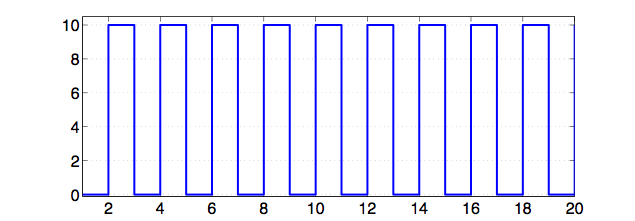
\includegraphics[scale=0.25]{100.png} 100\%\\
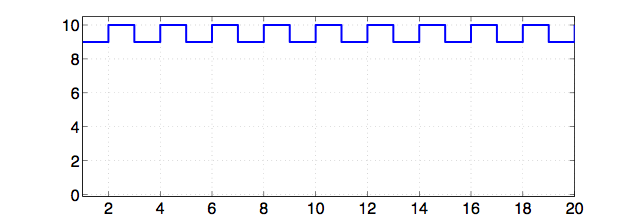
\includegraphics[scale=0.25]{10.png} 10\%
\end{frame}
%-----------------------------------------------------------------
\subsubsection{Signal Coding Methods}
\begin{frame}
\frametitle{Signal Coding Methods}
\begin{itemize}
\item Manchester coding:
\begin{itemize}
\item low-high transition = 0
\item high-low transition = 1
\end{itemize}
\item Modified Miller cding (delay encoding)
\begin{itemize}
\item Bit inversion \textbf{during} period denotes change in symbol.
\item Type of transition depends on location of inversion.
\item Beneficial as non-positive signal duration are short ensuring power transfer during data transmission.
\item Singal energy does not stay low for long.

\end{itemize}
\end{itemize}
\centerline{ 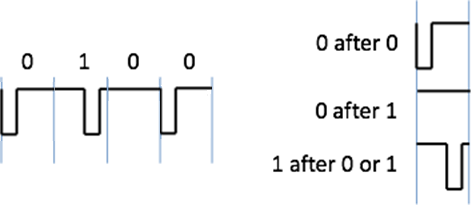
\includegraphics[scale=0.25]{modmil.png}}
\end{frame}
%----------------------------------------------------------------
\subsubsection{Configurations}
\begin{frame}
\frametitle{Configurations}
\begin{itemize}
\item Depends on the capability of the tag:
\begin{tabular}{|c|c|c|}
\hline
Speed & Active & Passive\\
\hline
\hline
424kb/s & Manchester (10\% modulation) & Manchester\\
\hline
212kb/s & Manchester & Manchester\\
\hline
106kb/s & Modified Miller (100\% modulation) & Manchester\\
\hline
\end{tabular}
\item Modfied Miller coding gives best protection against external modification.
\item Can only modify low-high transitions and so only 0 after 0 or 1 after 1 may be affected.
\end{itemize}
\end{frame}
%-----------------------------------------------------------------
\section{Summary}
\begin{frame}
\frametitle{Summary}
\begin{itemize}
\item NFC tags store data, NFC readers read the data from the tags.
\item Simplified network stack.
\item NFC is a standard of very short-range data transmission.
\item Active devices may power passive devices.
\item Operation very similar to other wireless network standards (i.e. IEEE 802.11).
\item Collision avoidance (half-duplex)
\item Carrier sense for existing RF field.
\end{itemize}
\end{frame}
%-----------------------------------------------------------------
\begin{frame} 
\Huge{\centerline{The End}}
\end{frame}
\end{document}